\documentclass[a4paper,12pt]{report}
\usepackage{graphicx}
\title{Membuat Aplikasi pada Orecle APEX}
\author{Nuha Hanifatul Khonsa'}
\date{ 7 November 2019}
\begin{document}


\maketitle

\section{Langkah dalam Pembuatan Aplikasi pada Orecle Apex}
\begin{enumerate}
    \item Hal pertama kita harus memiliki dokumen dalam bentuk excel seperti, Tabel Mahasiswa, Tabel Dosen, Tabel Matakuliah, Tabel Nilai, dan Table Jadwal. Lalu kita dapat membuka APEX online pada link https://apex.oracle.com/en/, lalu sign in dan masukkan data.
     \begin{center}
    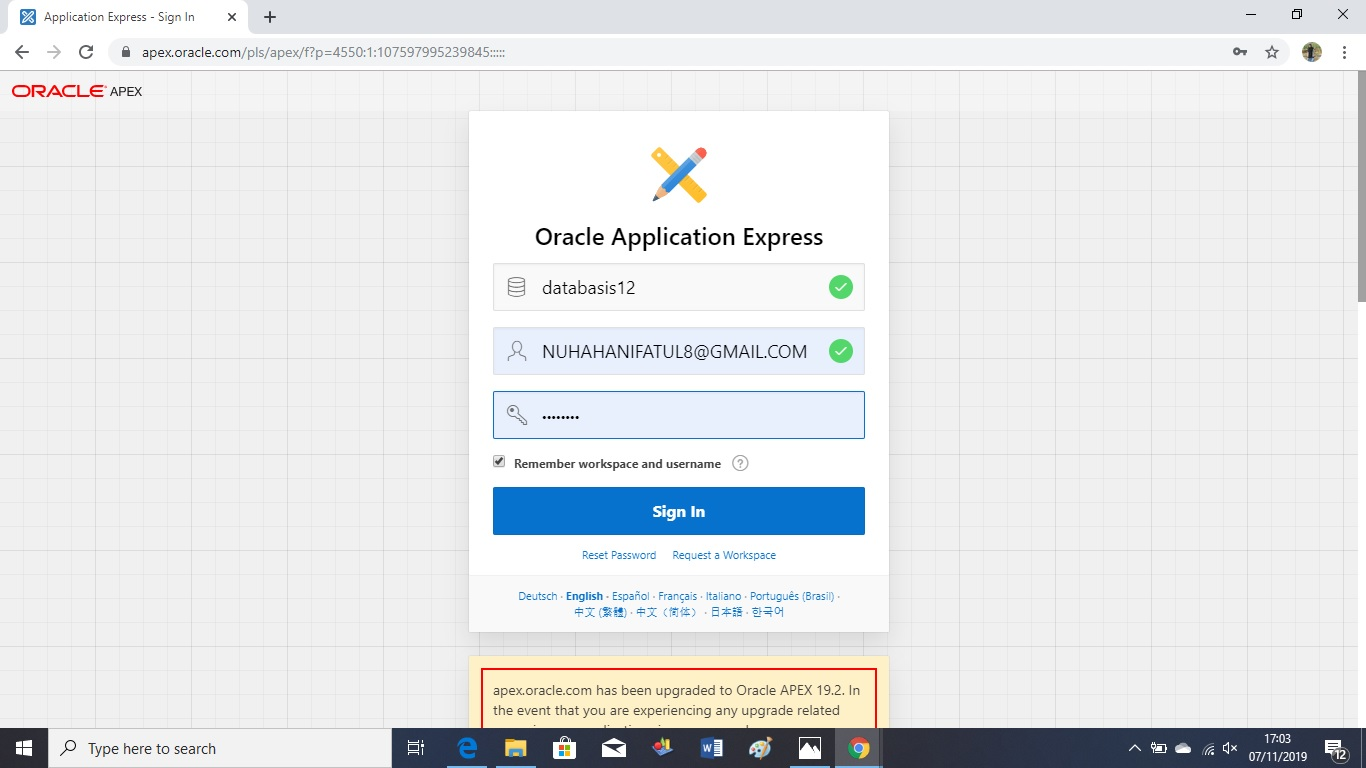
\includegraphics[width=11cm\textwidth]{figure/login.jpg}
    \end{center}
    \item Pilih APP Builder, Lalu pilih Create
     \begin{center}
    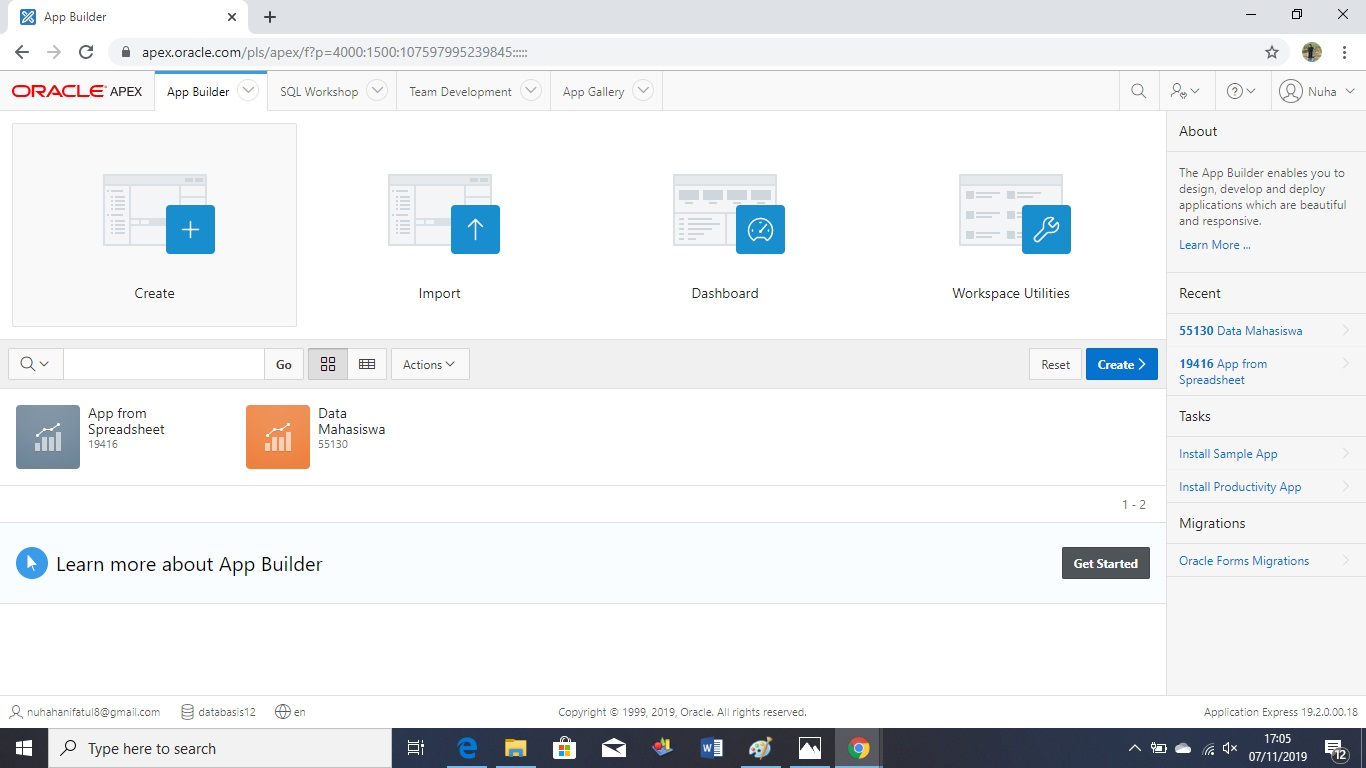
\includegraphics[width=11cm\textwidth]{figure/3.jpg}
    \end{center}
    \item Kemudian pilih from a file
     \begin{center}
    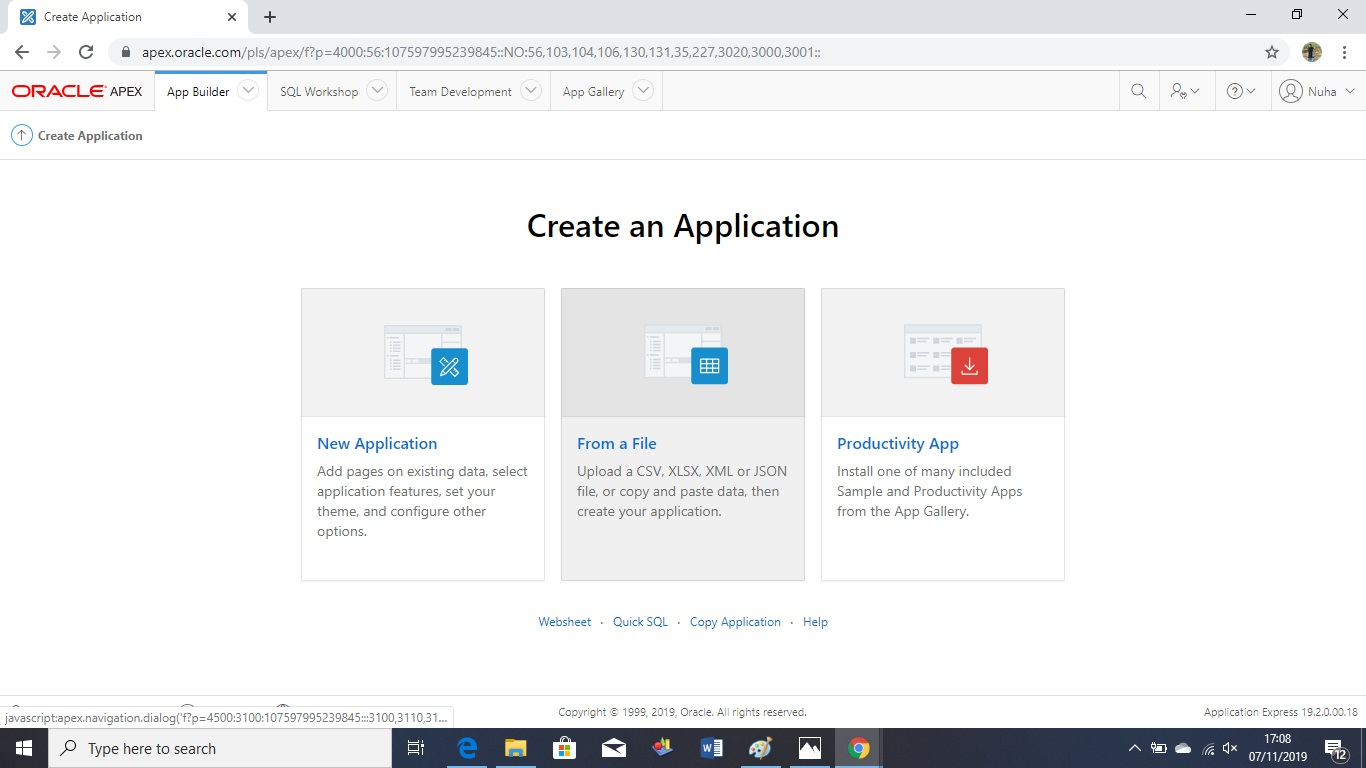
\includegraphics[width=11cm\textwidth]{figure/4.jpg}
    \end{center}
    \item Setelah itu kita dapat memilih upload file lalu Choose  File dan pilih data excel yang akan dimasukkan.
     \begin{center}
    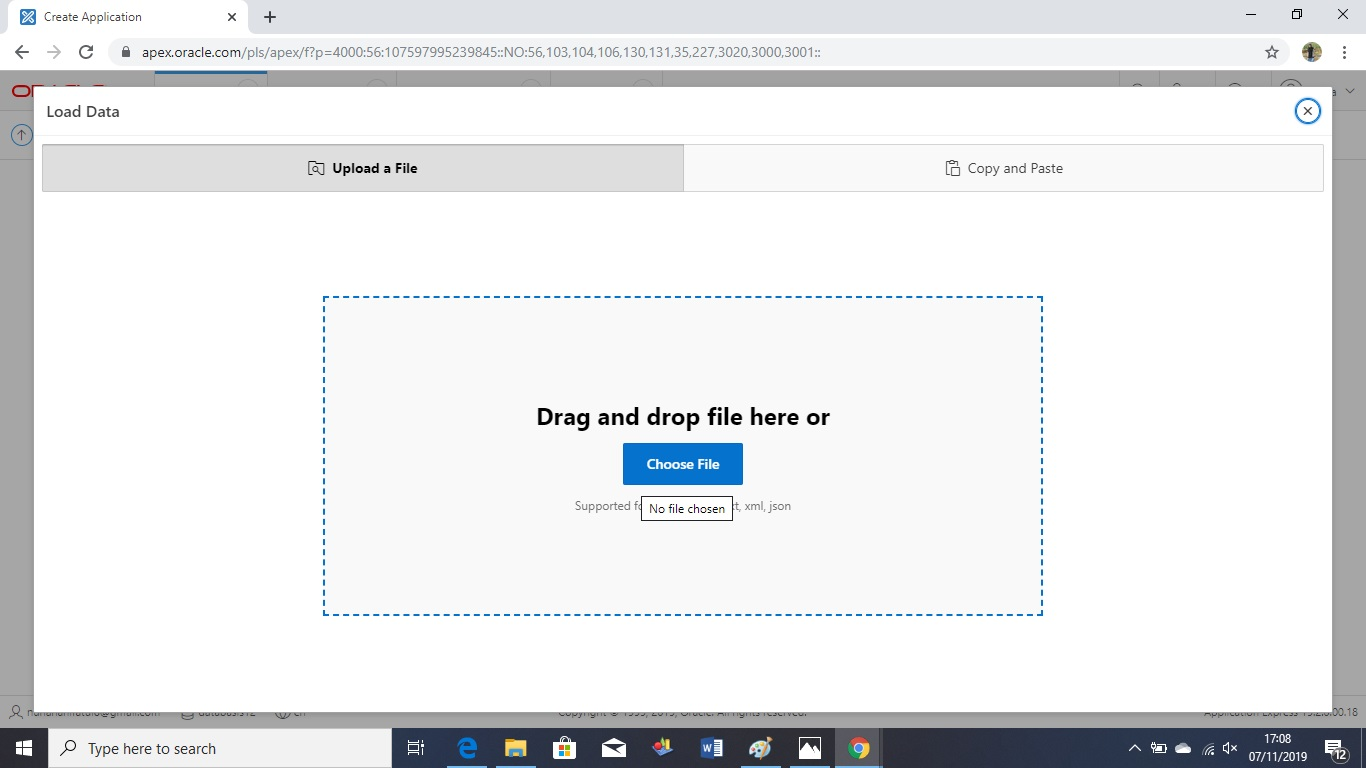
\includegraphics[width=11cm\textwidth]{figure/5.jpg}
    \end{center}
    \item Kemudian kita dapat mengisikan Table Name dan jika kita ingin mengecek isi dari table yang telah dimasukkan tadi kita dapat memilih configure. lalu kita load data
     \begin{center}
    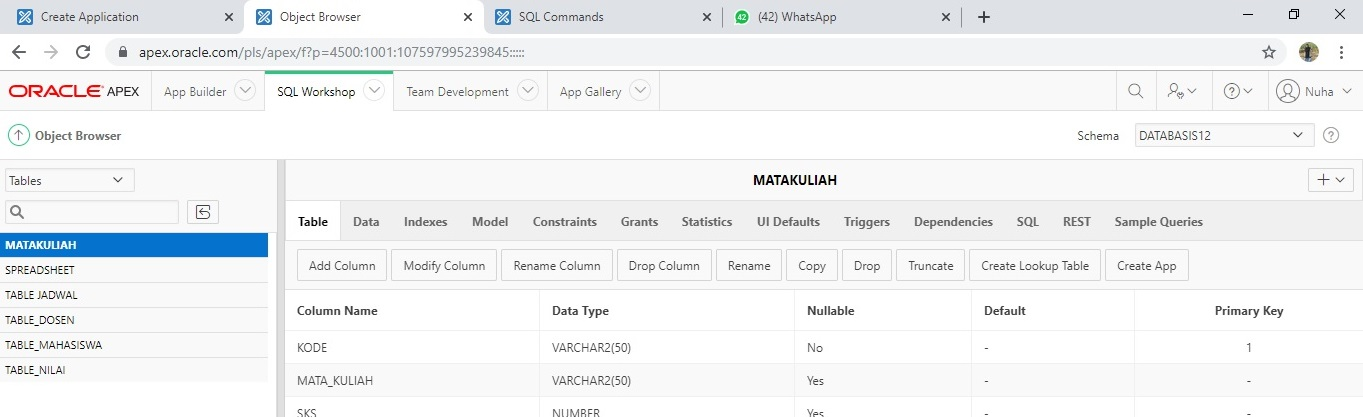
\includegraphics[width=11cm\textwidth]{figure/6.1.jpg}
    \end{center}
    \item Ulangi langkah dalam memasukkan data sehingga semua data telah terinputkan. Meliputi Table Mahasiswa, Table Dosen, Table Matakuliah, Table Nilai, dan Table Jadwal.Ini tampilan ketika semua table telah diinputkan, dan jangan lupa untuk menghapus ID pada tiap tabel dengan pilih Drop Colomn agar tidak terjadi eror.
    \begin{center}
    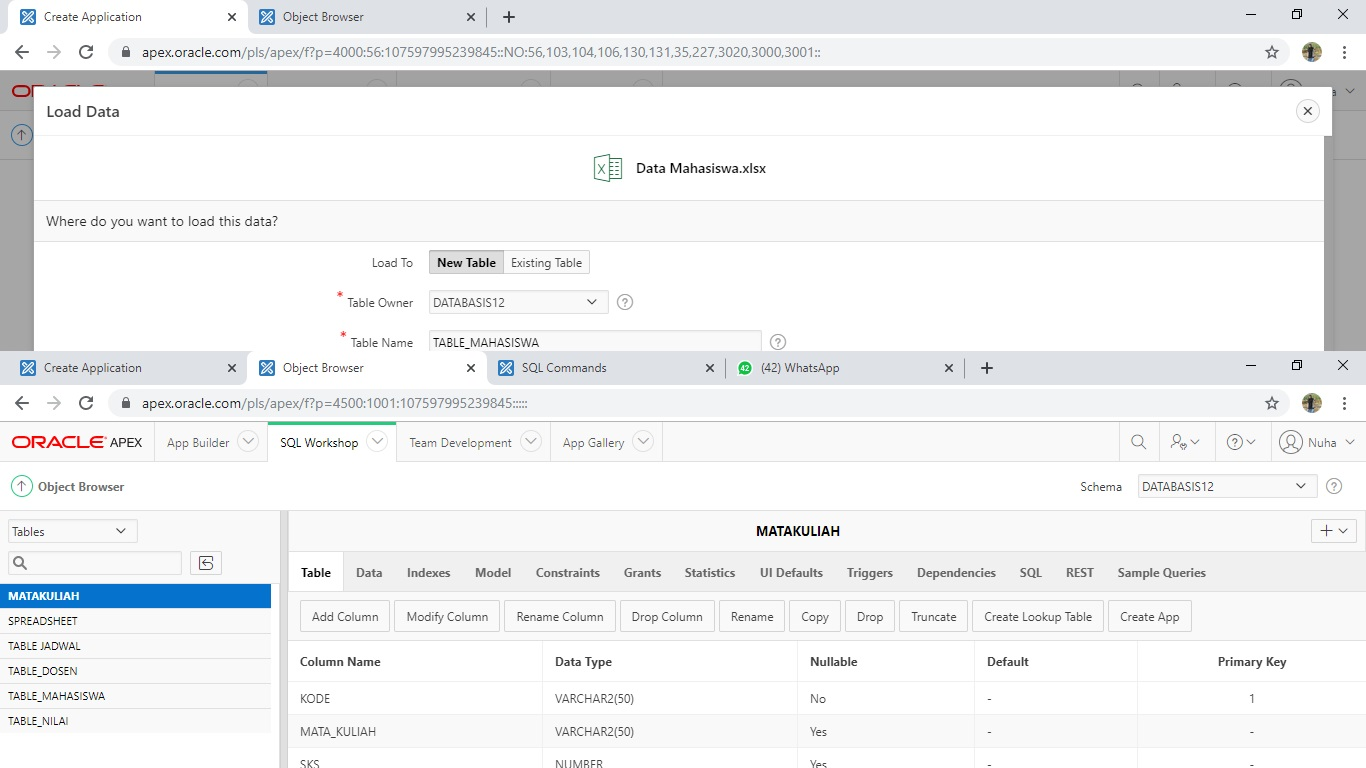
\includegraphics[width=11cm\textwidth]{figure/8.jpg}
    \end{center}
    \item Lalu buka SQL Commmand lalu masukkan perintah quary untuk memasukakkan primary dan foreign key pada tiap table
    \item Jika semua table telah mimiliki primary and foreign key kita dapat memilih klik app buiod lalu create dan New Aplikasi,
    \item Pada Create An Aplication masukkan nama aplikasi seperi Akademik Sederhana, Dan jangan lupa untuk memasukkan semua halaman dengan memilih add page lalu pilih FORM kemudian namai halaman dan pilih table yang ingin dimasukkan semisal, saya menamai halaman Mahasiswa jadi select table mahasiswa
     \begin{center}
    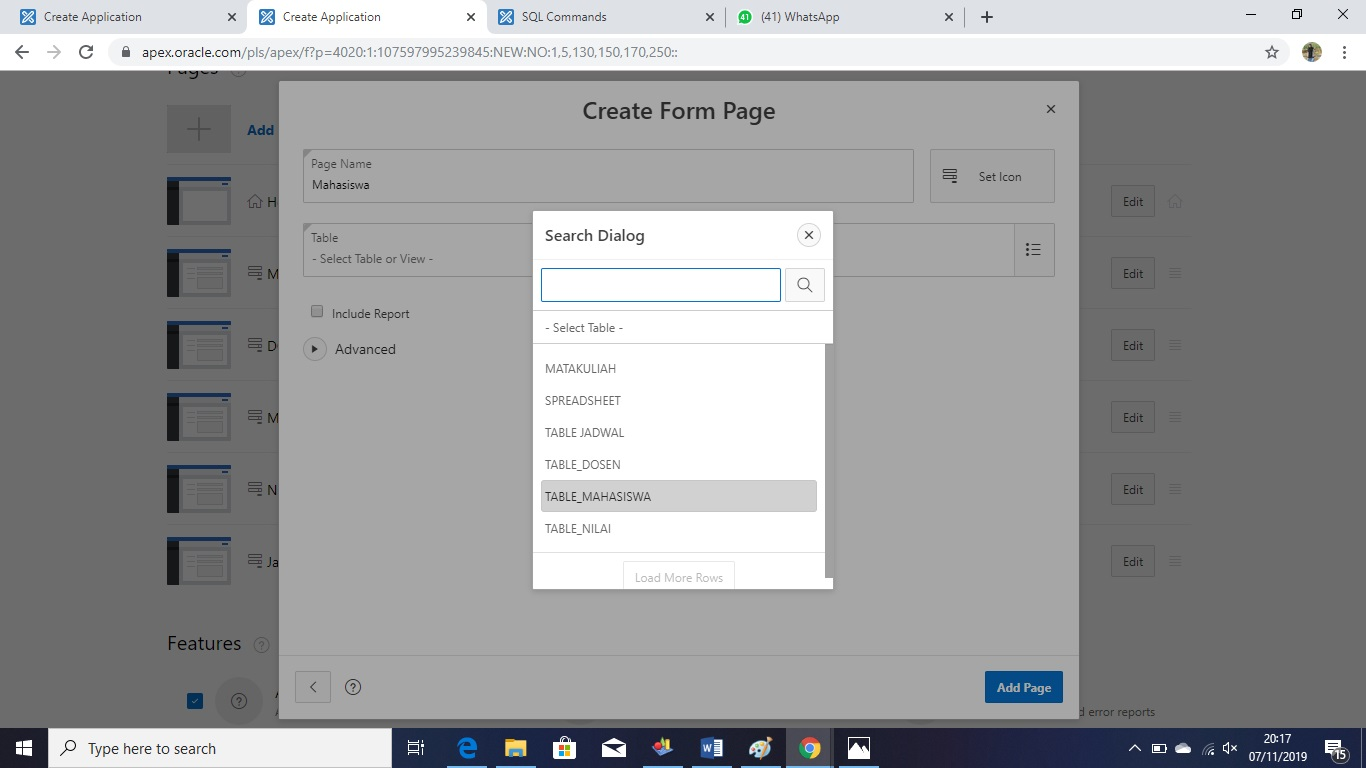
\includegraphics[width=11cm\textwidth]{figure/17.jpg}
    \end{center}
    \item saat page telah ditambahkan
     \begin{center}
    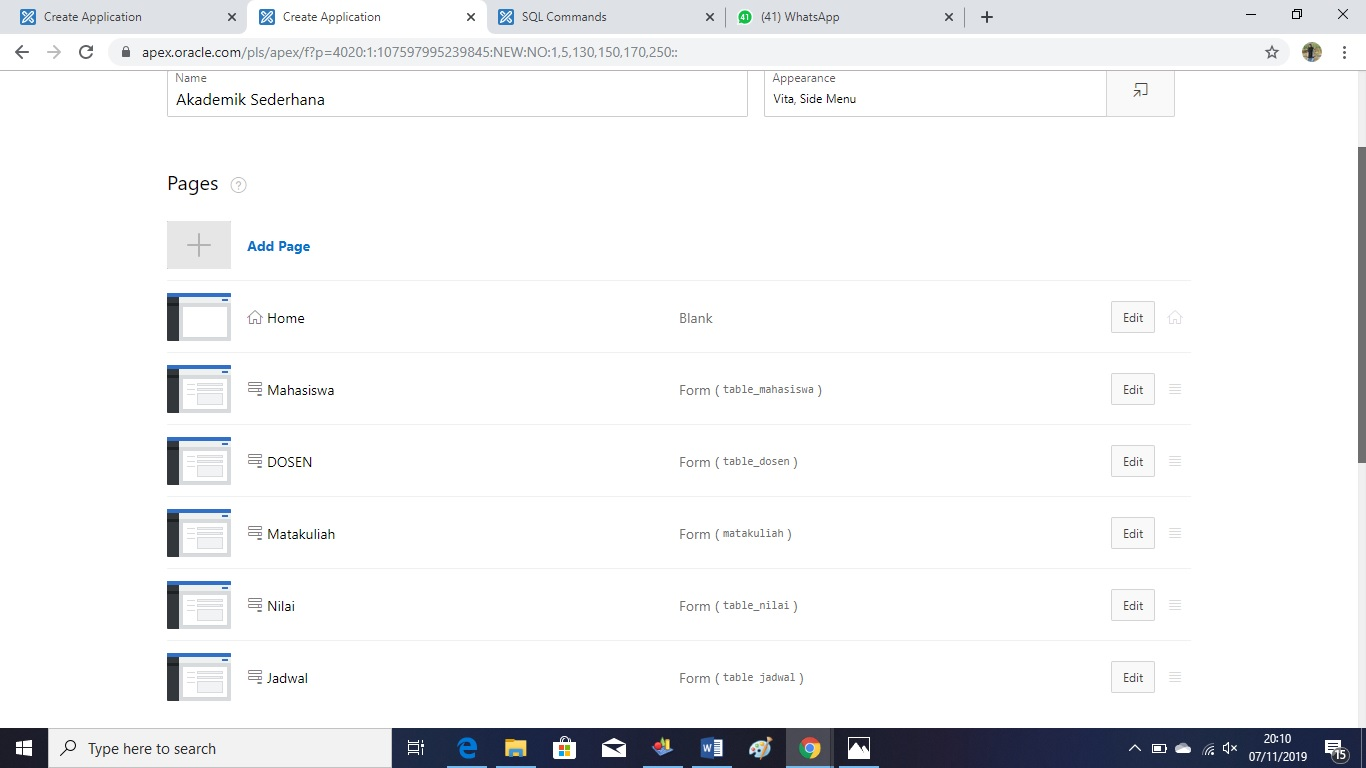
\includegraphics[width=11cm\textwidth]{figure/15.jpg}
    \end{center}
    \item pilih features dan chek all lalu create aplication
     \begin{center}
    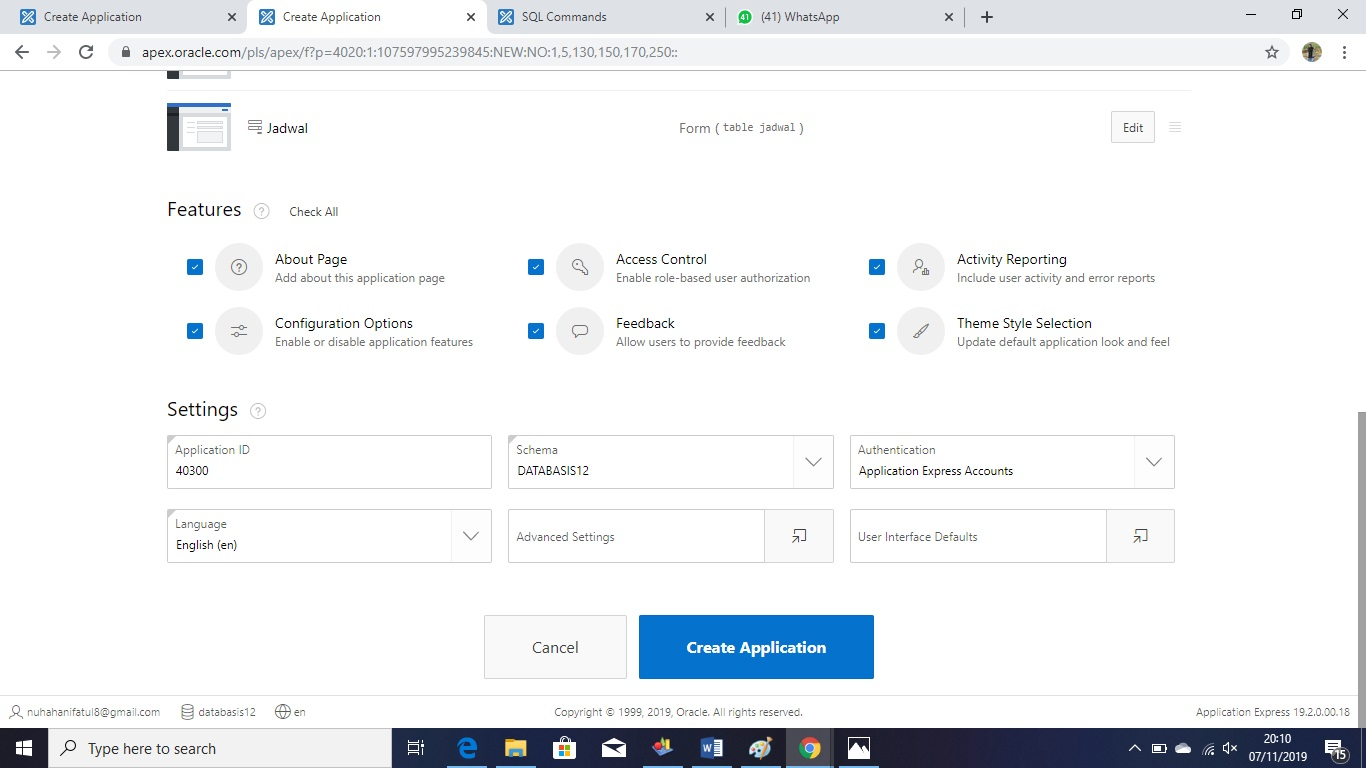
\includegraphics[width=11cm\textwidth]{figure/16.jpg}
    \end{center}
    \item Kemudian Run Aplikasi, lalu masukkan user credensial anda.
    \begin{center}
    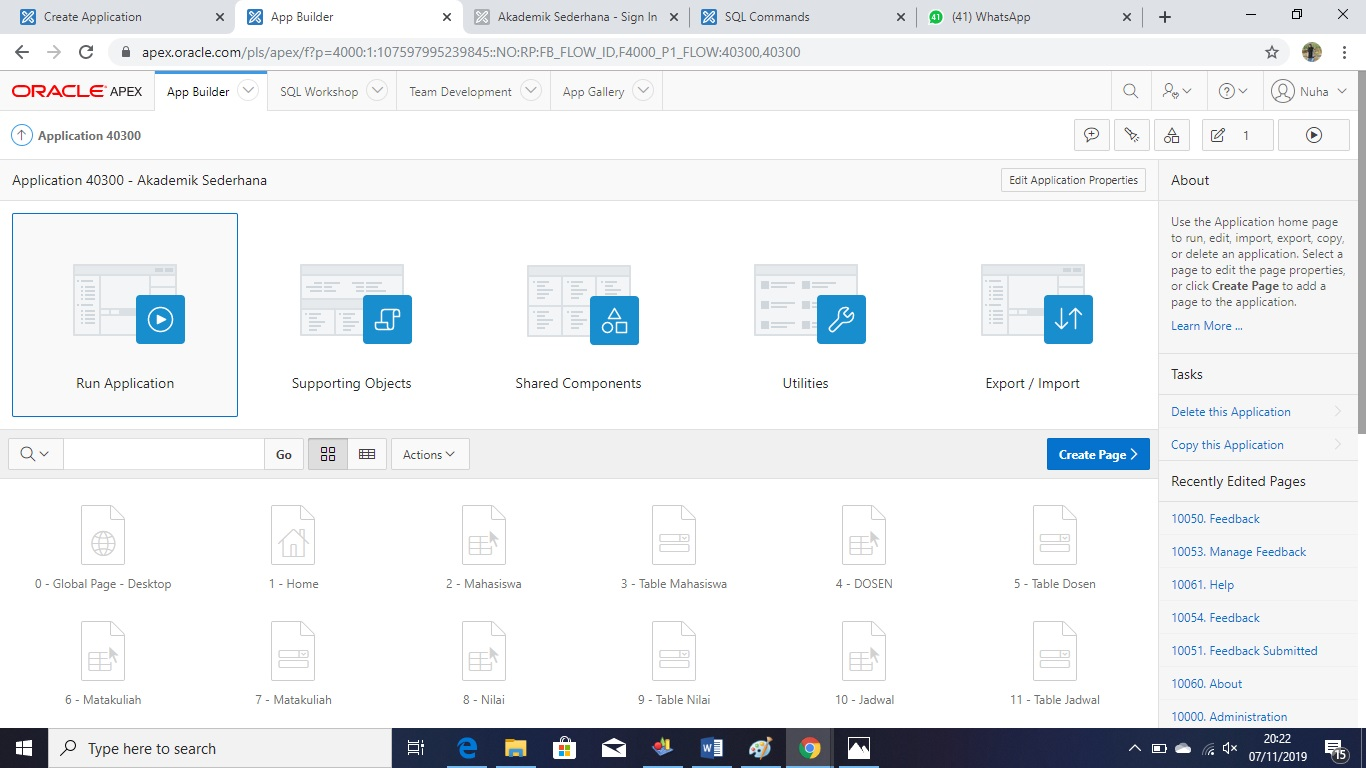
\includegraphics[width=11cm\textwidth]{figure/18.jpg}
    \end{center}
    \item Berikut ini home aplikasi dari akademik sederhana
    \begin{center}
    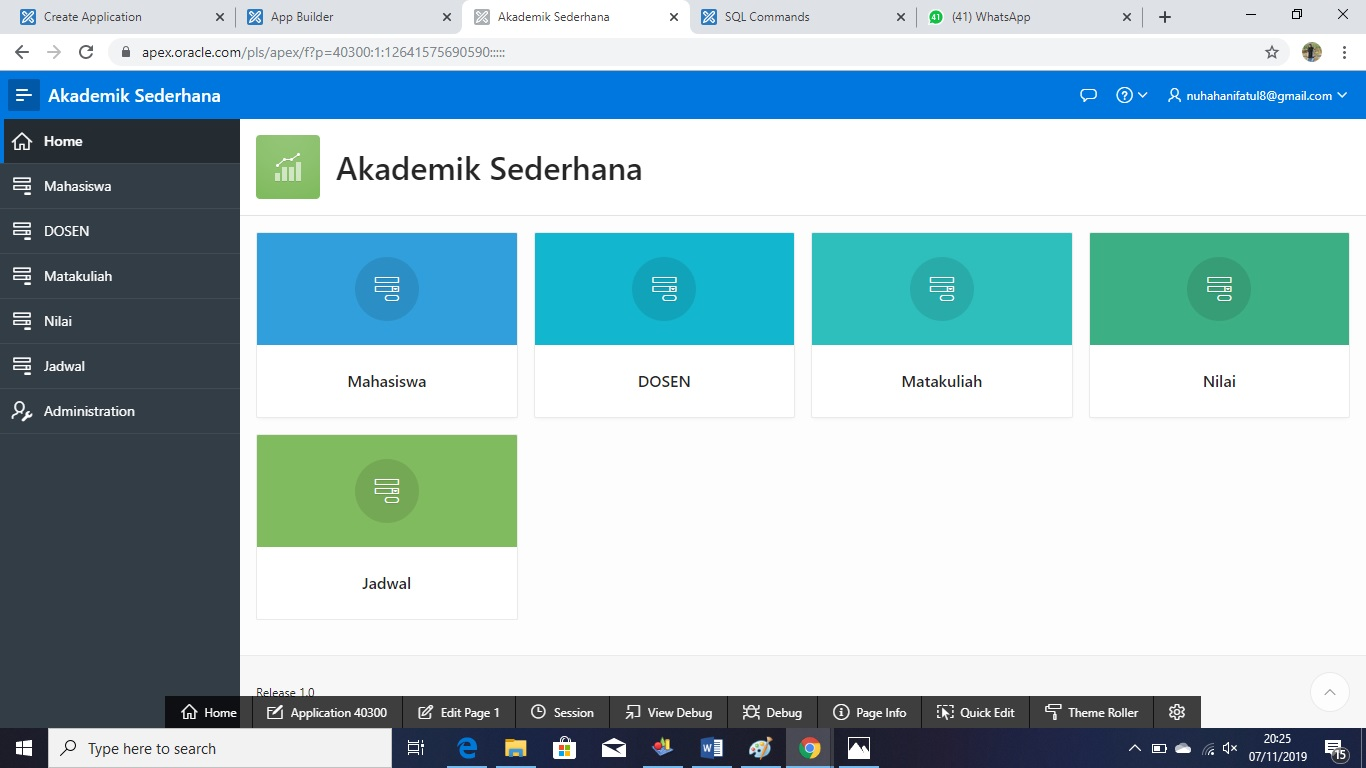
\includegraphics[width=11cm\textwidth]{figure/19.jpg}
    \end{center}
    \item https://apex.oracle.com/pls/apex/f?p=40300:2:12641575690590::NO:::
\end{enumerate}
\end{document}
